% =====================================================================
%  arXiv preprint — condensed from the master's thesis
%  Build:  tectonic -X compile main.tex
%  Self-contained: uses only standard TeX Live packages (no custom .sty),
%  which keeps the arXiv source package minimal.
% =====================================================================
\documentclass[11pt]{article}

\usepackage[utf8]{inputenc}
\usepackage[T1]{fontenc}
\usepackage[margin=1in]{geometry}
\usepackage{amsmath,amssymb}
\usepackage{booktabs}
\usepackage{graphicx}
\usepackage{multirow}
\usepackage{array}
\usepackage{caption}
\usepackage{microtype}
\usepackage[numbers,sort&compress]{natbib}
\usepackage{xcolor}
\usepackage[colorlinks=true,allcolors=blue!60!black,breaklinks=true]{hyperref}
\usepackage{url}

% --- light preprint styling (replaces a non-standard arxiv.sty) -------
\usepackage{titlesec}
\titleformat{\section}{\normalfont\large\bfseries}{\thesection}{0.6em}{}
\titleformat{\subsection}{\normalfont\normalsize\bfseries}{\thesubsection}{0.6em}{}
\captionsetup{font=small,labelfont=bf,skip=6pt}
\setlength{\parskip}{0pt}
\renewcommand{\arraystretch}{1.12}

\newcommand{\ie}{i.e.\ }
\newcommand{\eg}{e.g.\ }

% =====================================================================
\title{\bfseries Domain Adaptation of Lightweight Vision--Language Models\\
for Medical Visual Question Answering:\\
QLoRA Fine-Tuning with Autonomous Hyperparameter Optimization}

% TODO(author): confirm romanized name spellings against passport / prior publications.
%   "Dugki Min" is the given-family byline order; the university's own directory
%   lists the surname first as "Min, Dugki". Confirm which form the advisor uses
%   on his own publications before submitting -- a v1 cannot be withdrawn.
\author{%
  Taewook Hwang \qquad Dugki Min\\[2pt]
  Department of Convergence Information Technology, Major in Artificial Intelligence\\
  Graduate School of Information \& Telecommunications, Konkuk University\\
  Seoul, Republic of Korea\\[2pt]
  \texttt{taewook486@konkuk.ac.kr}
}
\date{}

% =====================================================================
\begin{document}
\maketitle

\begin{abstract}
We ask whether lightweight vision--language models (VLMs) can be adapted to
medical visual question answering (VQA) on consumer-grade GPUs, and answer it
with a three-stage study under a single evaluation protocol. Four open 2--3B
models (Qwen3-VL-2B, Qwen2.5-VL-3B, SmolVLM2-2.2B, Gemma4-E2B) are evaluated on
PathVQA, SLAKE and VQA-RAD across zero-shot baselines (12 conditions), QLoRA
fine-tuning (75 conditions), and a comparison of hyperparameter search
strategies (810 trials). Zero-shot accuracy differs significantly across models
(Cochran's $Q = 1904.28$, $\mathit{df} = 3$, $p < .001$), and the ranking
survives removal of samples flagged as likely pretraining exposure by
Min-$K$\% Probability. The effect of QLoRA is heterogeneous \emph{in direction}:
it significantly improves Qwen2.5-VL-3B ($d = +2.646$) and Qwen3-VL-2B
($d = +1.620$) yet significantly degrades SmolVLM2-2.2B ($d = -2.284$), and a
mixed-effects model pooling all four reports no effect ($p = .3629$) because the
opposing effects cancel. In autonomous hyperparameter search, an LLM agent
($0.4184$) performs significantly worse than Bayesian optimization ($0.4490$;
Mann--Whitney $U = 16.00$, $p = .0112$, $r = -0.68$) and is indistinguishable
from random search ($0.4186$), though all three automated strategies exceed the
manual configuration ($0.3776$). The agent's disadvantage traces not to proposal
quality but to a reduced effective budget caused by duplicate proposals ($12.5$
of $20$ unique configurations per repeat); a 200-trial re-experiment removing
the prompt--implementation inconsistency recovered uniqueness to $18.90$ of $20$
and dissolved the significant gap ($p = .1726$), yet still did not demonstrate
improvement ($p = .2387$). Notably, the variation observed when repeating an
identical configuration ($0.056$) exceeds the mean difference between strategies
($0.031$), a quantitative counterexample to comparing search methods from single
runs.

\end{abstract}

\section{Introduction}
\label{sec:intro}

Driven by the success of large language models (LLMs), vision--language models
(VLMs) that jointly understand images and text have advanced rapidly, led by
systems such as GPT-4V and Gemini. These general-purpose VLMs perform well on
question answering over natural images, but their performance tends to be limited
in domains requiring specialist knowledge, such as medical imaging, because they
lack an adequate grasp of medical terminology and of pathological and
radiological findings. At the same time, retraining large models from scratch is
not realistic in research and clinical environments with constrained GPU
resources. Parameter-efficient fine-tuning (PEFT) methods such as QLoRA
(quantized low-rank adaptation) \citep{dettmers2023qlora} have therefore
attracted attention as an alternative that makes domain-specific fine-tuning
feasible even on consumer-grade GPUs with 16--24\,GB of VRAM.

Applying a PEFT method such as QLoRA in practice, however, requires selecting a
number of hyperparameters --- LoRA rank, target modules, learning rate, and
others --- and the influence of these choices on final performance often remains
unexamined in a systematic way. Automating hyperparameter optimization (HPO) was
identified as an open problem for VLM PEFT in a 2024 NeurIPS survey. Beyond
traditional grid and random search \citep{bergstra2012random} or Bayesian
optimization (Optuna TPE) \citep{akiba2019optuna}, an autonomous search paradigm
has been proposed in which an LLM agent interprets prior experimental results on
its own and proposes the next configuration.

This paper empirically verifies the full process of adapting lightweight VLMs to
the medical imaging VQA (visual question answering) domain on consumer GPUs. We
demonstrate the feasibility of medical VQA domain adaptation for lightweight VLMs
on consumer-class GPUs (executed here on 24\,GB cards; applicable to the 16\,GB
class on the basis of measured VRAM); we systematically analyse how the principal
hyperparameters of QLoRA fine-tuning --- data scale, LoRA rank, and the scope of
target modules --- affect performance; and we verify whether autoresearch-style
autonomous hyperparameter search driven by an LLM agent delivers performance
competitive with Bayesian optimization while providing interpretable search
rationales. These aims are formalized as the three research questions in
Table~\ref{tab:rqs}.

\begin{table}[t]
\centering
\caption{Research questions and null hypotheses.}
\label{tab:rqs}
\small
\begin{tabular}{@{}p{0.05\textwidth}p{0.55\textwidth}p{0.30\textwidth}@{}}
\toprule
\# & Research question & Null hypothesis \\
\midrule
RQ1 & Do lightweight VLMs (2--3B) differ significantly across models in
zero-shot medical VQA performance? & $H_0$: no difference in VQA accuracy across
models \\
RQ2 & Does QLoRA fine-tuning significantly improve medical VQA performance? &
$H_0$: base $=$ fine-tuned performance \\
RQ3 & Does LLM-agent-based autonomous hyperparameter search achieve performance
competitive with Bayesian optimization (Optuna TPE) while providing interpretable
search rationales? & $H_0$: autoresearch $=$ Optuna (TPE) \\
\bottomrule
\end{tabular}
\end{table}

The null hypothesis for RQ3 was set against Optuna (TPE) rather than plain random
search because the justification for adopting LLM-based HPO --- natural-language
explanation of search rationale, use of prior knowledge to understand the
structure of the search space, and traceability of the reasons for configuration
changes --- holds only if such a method can compete with Bayesian optimization,
which is already established as a practical standard, rather than merely being
``better than random.'' Random search is retained solely as a lower-bound
reference. RQ1, RQ2, and RQ3 are verified against measured data in
Sections~4.1, 4.2, and 4.3 respectively, and the discussion cutting across all
three results is consolidated in Section~4.4.

The experimental scope is limited to four lightweight VLMs (Qwen3-VL-2B,
Qwen2.5-VL-3B, SmolVLM2-2.2B, Gemma4-E2B) and three public medical VQA datasets
(PathVQA, SLAKE, VQA-RAD). Models were selected on the criteria that QLoRA
fine-tuning was expected to be feasible within 16\,GB-class VRAM (confirmed
\emph{post hoc} at a measured maximum of 14.4\,GB, Section~\ref{sec:hardware})
and that the license permits free redistribution (Apache 2.0 / MIT). Datasets
were restricted to publicly accessible benchmarks in which clinical question
types are labelled.

\paragraph{Contributions.} This paper makes three contributions.
\begin{itemize}
\itemsep2pt
\item It provides three-stage empirical evidence on medical-domain adaptation of
lightweight VLMs under a single protocol, showing that performance and resource
consumption are not monotonically related and thereby offering a concrete basis
for model selection under resource constraints.
\item It quantifies the model-level heterogeneity of fine-tuning effects and
demonstrates how pooled analysis conceals opposing effects.
\item It reports a negative result for LLM-based autonomous optimization together
with a verification of its failure mechanism. Notably, the variation observed
when repeating an identical configuration (0.056) exceeded the mean difference
between strategies (0.031), constituting a quantitative counterexample to the
practice of comparing methods from single runs.
\end{itemize}

\section{Related Work}
\label{sec:related}

\paragraph{Lightweight vision--language models.}
A VLM combines an image encoder with an LLM so as to understand and generate
visual and linguistic information jointly. Early multimodal learning centred on
contrastive learning over image--text pairs to learn a shared embedding space; as
the instruction-following capability of LLMs advanced, the dominant approach
shifted to projecting image features into the input token space of an LLM and
using instruction tuning to acquire visual question answering and description
generation abilities. LLaVA \citep{liu2023llava} is a representative case in
which an open-source LLM was fine-tuned on visual instruction data generated by
GPT-4, and many subsequent VLM studies inherited this instruction-tuning
paradigm. Commercial large-scale VLMs such as GPT-4V and Gemini secure
general-purpose visual understanding through vast parameter counts and training
data, but their inference cost and deployment constraints limit their use on
consumer-grade hardware. The four models targeted here are all lightweight VLMs
in the 2--3B class released in 2025--2026, each pursuing parameter efficiency in
a different way. Qwen2.5-VL \citep{bai2025qwen25vl} is characterized by
dynamic-resolution processing, which adjusts the number of visual tokens
according to image size, and by an MRoPE extension that aligns temporal
information to absolute time. Its successor, Qwen3-VL, expanded into dense
(2B/4B/8B/32B) and mixture-of-experts (30B-A3B/235B-A22B) families and introduced
a ``thinking mode'' together with DeepStack-style multi-level fusion of visual
features. SmolVLM2 \citep{marafioti2025smolvlm} is an on-device-oriented
architecture combining a SigLIP image encoder with the SmolLM2 language model,
focusing on extremely low memory usage (5.2\,GB for video inference in the 2.2B
model). Gemma4-E2B is a mixture-of-experts-family structure that activates only
2.3B parameters at inference through per-layer embeddings (PLE) while exploiting
the expressive capacity of a 5.1B-class total parameter count.

\paragraph{Parameter-efficient fine-tuning.}
LoRA \citep{hu2022lora} freezes a pretrained weight matrix $W_0$ and learns an
approximation of its update $\Delta W$ as the product $BA$ of two low-rank
matrices $A \in \mathbb{R}^{r \times k}$ and $B \in \mathbb{R}^{d \times r}$, with
$r \ll \min(d,k)$. The forward pass is $h = W_0 x + BAx$, and since only $A$ and
$B$ are trained, the ratio of trainable to total parameters can be reduced
dramatically. The rank $r$ governs the trade-off between expressive capacity and
parameter efficiency, while alpha scales $\Delta W$ (multiplying $BAx$ by
$\alpha/r$). QLoRA \citep{dettmers2023qlora} combines LoRA with 4-bit
quantization to reduce VRAM usage further, through (1) 4-bit NormalFloat (NF4)
quantization optimized for normally distributed weights, (2) double quantization,
which quantizes the quantization constants themselves, and (3) a paged optimizer
that offloads GPU memory spikes to the CPU; the original paper showed that this
allows fine-tuning of a 65B-class model on a single 48\,GB GPU while maintaining
performance close to full 16-bit fine-tuning. Other PEFT methods include partial
fine-tuning, prefix tuning, and adapter insertion between transformer layers.
Compared with these, the advantages of the LoRA family are that $BA$ can be
merged into $W_0$ at inference time so that no additional latency is incurred,
and that adapters can be stored and swapped independently, allowing a single base
model to be reused across multiple tasks. We adopt LoRA/QLoRA because these two
advantages are particularly favourable for the repeated hyperparameter search
conducted on consumer GPUs.

\paragraph{Medical VQA benchmarks and medical-specialised models.}
Medical VQA is the task of generating a correct answer given a medical image (a
pathology tissue slide, a radiological image, and so on) together with a
natural-language question; unlike general-domain VQA it requires both an
understanding of specialist medical terminology and fine-grained visual grounding
of imaging findings. Question types divide broadly into closed-ended questions
answered yes/no or by selecting among options and open-ended questions requiring
free-form answers, and the two types differ greatly in scoring method and
difficulty. PathVQA \citep{he2020pathvqa} provides 32,799 question--answer pairs
over 4,998 pathology tissue images extracted from pathology textbooks and the
PEIR digital library, organized into seven question types modelled on the
American Board of Pathology certification examination format. SLAKE
\citep{liu2021slake} combines 14,028 bilingual English--Chinese question--answer
pairs over 642 radiology/CT images with a medical knowledge graph of 5,232
knowledge triplets. VQA-RAD \citep{lau2018vqarad} was the first dataset to
collect questions that clinicians naturally raised while viewing radiological
images (CT/MRI/X-ray), containing roughly 3,500 question--answer pairs over 315
images. Attempts to specialize general-purpose VLMs for the medical domain divide
into large-scale retraining and adaptation approaches. LLaVA-Med
\citep{li2023llavamed} generated GPT-4-based instruction data from large-scale
biomedical figure--caption data in PubMed Central and adapted general-purpose
LLaVA to the biomedical domain through curriculum learning. Med-Flamingo
\citep{moor2023medflamingo} performed continued pretraining of OpenFlamingo-9B on
image--text data from medical papers and textbooks, acquiring the ability to
adapt to medical VQA from only a few examples. CheXagent
\citep{chen2024chexagent} is a foundation model composed of a clinical LLM, a
visual encoder, and a cross-modal bridge network specialized for chest X-ray
interpretation. These prior studies commonly target models on the scale of
billions to hundreds of billions of parameters and presuppose either continued
pretraining on large biomedical corpora or the generation of large-scale
instruction data; by contrast, we fine-tune 2--3B-class lightweight models with
QLoRA using only small domain datasets (thousands to tens of thousands of
samples).

\paragraph{Hyperparameter optimization, from random search to LLM agents.}
The simplest HPO method is grid search, whose required number of evaluations
grows exponentially with the dimensionality of the search space. Bergstra and
Bengio \citep{bergstra2012random} showed theoretically and empirically that
random sampling of combinations can yield substantially better --- or equivalent
--- performance than grid search within the same computational budget, because
the effective dimensionality of the hyperparameters that actually influence
performance is often low. Bayesian optimization constructs a probabilistic
surrogate model of the objective from previous evaluations and selects the next
evaluation point accordingly. Optuna \citep{akiba2019optuna}, used as the control
here, adopts the tree-structured Parzen estimator (TPE) algorithm and provides a
define-by-run API together with efficient pruning strategies. Among
early-stopping-based methods, Hyperband \citep{li2018hyperband} formulates HPO as
a pure-exploration bandit problem by repeatedly applying successive halving,
allocating little resource to unpromising configurations and progressively more
to promising ones; for this to hold there must be a significant rank correlation
between the early learning curve and final converged performance. In contrast to
Bayesian optimization, which relies on a numerical surrogate model, a scheme in
which an LLM agent directly interprets previous experimental logs and proposes
the next configuration through natural-language reasoning has recently been
discussed as a new alternative. Its theoretical distinctions are three: the LLM
can transfer knowledge across different tasks and architectures by drawing on
domain knowledge acquired during pretraining; unlike Bayesian optimization, which
treats individual hyperparameters as independent variables, it can understand
interactions among hyperparameters structurally on the basis of prior knowledge;
and it records the reason for changing a configuration explicitly in natural
language, providing interpretability and traceability. This is, however, less an
established standard methodology than one instance of an emerging research
current on the use of LLM agents for automating scientific experimentation.

\paragraph{What distinguishes this work.}
Research on medical-specialized VLMs generally presupposes large models and large
domain datasets; research on PEFT methodology concentrates on verifying parameter
efficiency in general domains; and research on HPO automation has rarely compared
LLM-agent-based methods directly against established Bayesian optimization on the
same task. At the intersection of these three currents --- consumer GPU
environment, lightweight VLMs, QLoRA domain adaptation, and LLM-based autonomous
HPO --- this paper verifies the zero-shot and fine-tuned medical VQA performance
of lightweight VLMs with statistical rigour (RQ1, RQ2) under a single protocol
spanning all three stages, and validates the practical value of
autoresearch-style autonomous search by comparing it directly against Optuna
(TPE) (RQ3), reporting a negative result together with a verified failure
mechanism.

\section{Method}
\label{sec:method}

\subsection{Overview of the research design}
\label{sec:design}

The study is designed as empirical research that verifies medical VQA domain
adaptation of lightweight VLMs sequentially through a three-phase experiment.
Phase~1 measures the zero-shot performance of the four models before fine-tuning
in order to answer RQ1 (differences across models). Phase~2 applies QLoRA
fine-tuning to verify RQ2 (the effect of fine-tuning) while simultaneously
exploring the optimal QLoRA configuration (data scale, LoRA rank, target modules)
through ablation studies. Phase~3 takes the optimal configuration identified in
Phase~2 as its starting point and compares four HPO strategies --- Manual, Random
Search, Optuna (TPE), and Autoresearch --- to verify RQ3 (the competitiveness of
autonomous search). Each phase has a sequential structure in which the results of
the preceding phase (best model, optimal QLoRA configuration) become fixed
conditions for the next.

\subsection{Experimental environment}
\label{sec:hardware}

All experiments reported here were conducted on a cloud GPU service (RunPod).
Phases~1 and 2 used an RTX 4090 (24\,GB VRAM) instance and Phase~3 an RTX 3090
(24\,GB VRAM) instance. The change of GPU in Phase~3 was not a design choice but
the result of securing whatever instance was available under tightened budget
constraints. Both are consumer-class cards with 24\,GB of VRAM, and every Phase~3
trial ran on the same 3090 instance, so the hardware conditions of the strategy
comparison were controlled. A local workstation (RTX 5060 Ti 16\,GB $+$ RTX 4060
8\,GB, Ryzen 5 5600X, 32\,GB RAM) was used only for a preliminary smoke test to
size the Phase~3 execution; none of the figures reported in this paper were
produced in the local environment.

Feasibility in the 16\,GB-class environment targeted by this work was confirmed
\emph{from measured VRAM usage rather than by execution on such a card}. Peak
VRAM during Phase~2 QLoRA training was at most 14,373\,MB across the four models
(Gemma4-E2B), within the 16\,GB limit, while the other three models required only
4,015--7,943\,MB.

Model loading and QLoRA fine-tuning used the HuggingFace \texttt{transformers}
library together with the \texttt{unsloth} backend for accelerated 4-bit
quantized training, with LoRA adapters configured through the \texttt{peft}
library. The Bayesian optimization control in Phase~3 used \texttt{Optuna} (TPE
sampler), and experiment management and logging used \texttt{wandb}. BERTScore
computation for scoring open-ended responses used the \texttt{bert-score} library
(roberta-large / BioBERT backbones), and statistical analysis used \texttt{scipy}
and \texttt{statsmodels} (mixed-effects model). The LLM agent of the Autoresearch
strategy calls the Anthropic Claude API.

\subsection{Target models and datasets}
\label{sec:models}

The four models examined and the grounds for their selection are given in
Table~\ref{tab:models}. The selection criteria were threefold: (1) QLoRA
fine-tuning must be feasible within 16\,GB of VRAM (an \emph{a priori}
expectation, confirmed \emph{post hoc} from measured peak VRAM,
Section~\ref{sec:hardware}); (2) the license must be Apache 2.0 or MIT so that
research use is unrestricted; and (3) the model must have sufficient community and
framework support. Gemma4-E2B was included because its mixture-of-experts-family
PLE technique activates only 2.3B parameters at inference while providing
5.1B-class expressive capacity.

\begin{table}[t]
\centering
\caption{Target models.}
\label{tab:models}
\small
\begin{tabular}{@{}llll@{}}
\toprule
Model & Parameters & Architectural features & Expected QLoRA VRAM \\
\midrule
Qwen3-VL-2B    & 2B   & Thinking mode, DeepStack             & $\sim$8--10\,GB \\
Qwen2.5-VL-3B  & 3B   & Dynamic resolution, OCR in 19 languages & $\sim$8--10\,GB \\
SmolVLM2-2.2B  & 2.2B & HuggingFace lightweight VLM          & $\sim$8--10\,GB \\
Gemma4-E2B     & 2.3B (active) / 5.1B (total) & PLE (per-layer embeddings), Apache 2.0 & $\sim$12--14\,GB \\
\bottomrule
\end{tabular}
\end{table}

The three public medical VQA datasets are summarized in
Table~\ref{tab:datasets}. Each dataset was used with its official
train/val/test split unchanged, and all reported accuracies are computed on the
\emph{test} split only. Because the size of a distributed copy can differ from
the figure reported in the dataset's original paper, Table~\ref{tab:datasets}
separates the three quantities that are easy to conflate: the size reported by
the source publication, the size of the copy we actually obtained, and the
number of items each model was actually evaluated on.

\begin{table}[t]
\centering
\caption{Target datasets. ``Published'' is the QA-pair count reported by the
dataset's own paper; ``Obtained'' is the total size of the distributed copy used
here; ``Evaluated'' is the test-split size on which every reported accuracy is
computed. No subsampling was applied --- the evaluated counts are the full test
splits.}
\label{tab:datasets}
\small
\begin{tabular}{@{}llrrrl@{}}
\toprule
Dataset & Source distribution & Images & Published & Obtained & Evaluated \\
\midrule
PathVQA & \texttt{flaviagiammarino/path-vqa}      & 4,998 & 32,799 & 32,632 & 6,719 \\
SLAKE   & \texttt{mdwiratathya/SLAKE-vqa-english} & 642   & 14,028 & 7,033  & 1,061 \\
VQA-RAD & \texttt{flaviagiammarino/vqa-rad}       & 315   & 2,248  & 2,244  & 451 \\
\bottomrule
\end{tabular}
\end{table}

PathVQA covers pathology tissue images with seven question types; SLAKE and
VQA-RAD cover radiology and CT/MRI/X-ray images. All three mix open-ended and
closed-ended questions. Note that the SLAKE distribution used here is the
English-only release: the 14,028 figure published for SLAKE counts its bilingual
English--Chinese pairs, whereas the copy obtained for these experiments contains
the English half alone.

\paragraph{Contamination control.}
PathVQA (2018), SLAKE (2021), and VQA-RAD (2018) were all released before the
pretraining cut-off of the target models (2025--2026), so the possibility of
pretraining data contamination cannot be excluded. We measure such contamination
actively using the Min-$K$\% Probability attack \citep{shi2024minkprob}. The mean
token-level log-probability of the lowest $K$\% ($K = 20$) of tokens in each
sample's gold answer text is used as the contamination indicator --- on the
theory that samples exposed during pretraining exhibit higher mean probability
--- and samples in the top 5\% within a dataset are classified as suspected
contamination, after which the principal conclusion (RQ1) is re-verified on the
reduced sample set with those samples removed. The interpretation criteria are
that a difference of less than 1\,\%p between original and reduced results is
deemed robust, 1--5\,\%p is stated as a limitation, and more than 5\,\%p requires
reconsideration of the conclusion.

\subsection{Phase 1: zero-shot baseline evaluation}
\label{sec:phase1}

Zero-shot performance before fine-tuning was measured for $4$ models $\times$ $3$
datasets $=$ 12 conditions. Because evaluation uses greedy decoding it is
deterministic: changing the seed does not change the result, so repeated trials
are meaningless. Evaluation therefore used a single seed (42), and uncertainty is
reported as a bootstrap 95\% confidence interval over the per-sample
correct/incorrect decisions of each condition. Since the four models are
evaluated on an identical test set, comparison across models has a paired
structure; accordingly, Cochran's $Q$ test (binary correctness on a shared test
set, $H_0$: equal accuracy) and pairwise McNemar post-hoc tests with Bonferroni
correction were used instead of ANOVA, which assumes independent samples. The
measured metrics are closed-ended accuracy (multiple choice), open-ended accuracy
(gold-token matching) together with BERTScore F1 (roberta-large), bootstrap 95\%
CIs for each accuracy, response time (ms per item), and peak VRAM (MB).

\subsection{Phase 2: QLoRA fine-tuning}
\label{sec:phase2}

The base QLoRA configuration applied to every Phase~2 condition is given in
Table~\ref{tab:qlora}. The training budget targeted 3 epochs, but a ceiling of
\texttt{max\_steps}~$=500$ (samples\_seen fixed at 4,000 per condition) was
imposed because of cloud GPU time and cost constraints. Since the training volume
is fixed regardless of dataset size, the small VQA-RAD receives roughly 2 epochs
or more while the medium SLAKE and large PathVQA receive less than 1 epoch; this
asymmetry is a stated limitation of the study and is carried into the
interpretation of the results.

\begin{table}[t]
\centering
\caption{Base QLoRA configuration (Phase 2).}
\label{tab:qlora}
\small
\begin{tabular}{@{}ll@{}}
\toprule
Parameter & Value \\
\midrule
Quantization    & NF4 (4-bit NormalFloat) \\
LoRA rank       & 64 (determined by Ablation B) \\
LoRA alpha      & 128 \\
LoRA dropout    & 0.05 \\
Target modules  & all-linear (determined by Ablation C) \\
Learning rate   & 2e-4 \\
Batch size      & 1 (gradient accumulation 8, effective batch $=$ 8) \\
Optimizer       & paged\_adamw\_8bit \\
\bottomrule
\end{tabular}
\end{table}

The experimental conditions are $4$ models $\times$ $3$ datasets $=$ 12
conditions, each repeated 3 times (seeds 42/123/456). The values LoRA rank $=64$
and target $=$ all-linear were fixed on the basis of three ablation studies, each
with PathVQA and Qwen3-VL-2B held fixed: Ablation~A (effect of data size) varies
the training-data ratio over 5/10/25/50/100\%; Ablation~B (effect of LoRA rank)
varies rank $\in \{4, 8, 16, 32, 64\}$; and Ablation~C (effect of target modules)
compares $\{$q/v\_proj$\}$ versus $\{$q/k/v/o\_proj$\}$ versus
$\{$all-linear$\}$.

Catastrophic forgetting is measured in two ways. (A) Change in general
capability: the rate of accuracy decrease before and after fine-tuning is
measured on a VQAv2 validation subset (2,000 samples) across all 12 conditions.
(B) Cross-dataset generalization within the medical domain: evaluation on a
dataset other than the training dataset (for example, train on PathVQA $\to$
evaluate on SLAKE/VQA-RAD), giving $12$ conditions $\times$ $2$ cross-datasets
$=$ 24 additional evaluations. Because PathVQA (pathology) and SLAKE/VQA-RAD
(radiology) differ in image domain itself, the results of (B) are interpreted as
a domain-generalization gap rather than as catastrophic forgetting in the strict
sense.

\subsection{Phase 3: autonomous hyperparameter optimization}
\label{sec:phase3}

The hyperparameter search space shared by the four strategies is given in
Table~\ref{tab:searchspace}. The four strategies compared are Manual (the
researcher's default values, one run), Random Search (random sampling), Optuna
TPE (Bayesian optimization), and Autoresearch (autonomous search by an LLM
agent). Autoresearch repeats a loop that (1) reads the previous experimental
results (\texttt{results.tsv}), (2) proposes the next configuration together with
a natural-language rationale (\texttt{config.yaml} $+$ \texttt{rationale.md}),
(3) performs a git commit, (4) runs fixed training, (5) evaluates on the
validation set, and (6) retains the configuration if performance improves and
discards it otherwise.

\begin{table}[t]
\centering
\caption{Phase 3 hyperparameter search space.}
\label{tab:searchspace}
\small
\begin{tabular}{@{}lll@{}}
\toprule
Parameter & Search range & Type \\
\midrule
lora\_rank        & $\{4, 8, 16, 32, 64\}$        & Discrete \\
lora\_alpha       & rank $\times \{1, 2, 4\}$     & Discrete \\
learning\_rate    & $[1\mathrm{e}{-5},\ 5\mathrm{e}{-4}]$ & Continuous (log scale) \\
batch\_size       & $\{1, 2, 4\}$                 & Discrete \\
grad\_accum\_steps & $\{4, 8, 16\}$               & Discrete \\
warmup\_ratio     & $[0.0,\ 0.1]$                 & Continuous \\
weight\_decay     & $[0.0,\ 0.1]$                 & Continuous \\
lora\_targets     & $\{$minimal, medium, full$\}$ & Categorical \\
\bottomrule
\end{tabular}
\end{table}

All trials share the same model (the best model from Phase~2), the same dataset
(PathVQA), and a fixed \texttt{max\_steps}~$=200$ in order to control training
volume; the wall-clock ceiling \texttt{time\_budget\_min} serves as a safety
device to prevent pathological combinations rather than as an experimental
control variable. The original design called for Manual 10 $+$ Random Search 400
$+$ Optuna 400 $+$ Autoresearch 400 $=$ 1,210 trials in total (40 trials per
strategy $\times$ 10 independent repeats). A preliminary smoke test conducted
solely to size the execution indicated on a wall-clock basis --- counting not
only training but also validation and final test evaluation time --- that the
original scale would require roughly 24--25 days even with two GPUs in parallel.
The number of repeats (10), which is the unit of statistical testing and the
basis of run-level statistical power, was therefore preserved, while the number
of search trials per strategy was reduced from 40 to 20, halving the total time
to approximately 12.8 days. The execution scale of the four-strategy comparison
is thus Manual 10 $+$ Random Search 200 $+$ Optuna 200 $+$ Autoresearch 200 $=$
610 trials in total (20 trials per strategy $\times$ 10 independent repeats).
This reduction carries the trade-off of halving the diversity of hyperparameter
combinations explored per strategy, but it does not affect the validity of the
run-level statistical tests based on 10 independent repeats.

In addition, a 200-trial configuration-consistency re-experiment
(Autoresearch-v2) was conducted separately. This is not part of the four-strategy
same-condition comparison but a follow-up intervention designed to test whether
the duplicate-proposal phenomenon dissolves once the prompt--implementation
inconsistencies are removed. The search space, model, dataset,
\texttt{max\_steps}, and repetition count were held identical to the original,
and only the five configuration inconsistencies were corrected; the original
condition was preserved intact for reproducibility. The total execution scale of
Phase~3 is 810 trials.

Statistical verification is performed only at the run level, not at the trial
level. Because Autoresearch and Optuna are sequential optimizers, trials within
the same run are dependent (the result of trial $t$ influences the proposal at
$t+1$), violating the assumption of independent observations. The unit of testing
is the 10 final performance values obtained from the 10 independent repeats of
each strategy, analysed with the Kruskal--Wallis test (four-group comparison),
the Mann--Whitney $U$ test (pairwise, Autoresearch vs.\ Optuna), and BCa
bootstrap 95\% CIs. Trial-level data are used only for visualization such as
anytime performance curves.

\subsection{Evaluation metrics and statistical analysis}
\label{sec:stats}

\paragraph{Dual reporting of BERTScore.}
Open-ended responses are reported with both exact match and BERTScore F1. The
general-purpose criterion (roberta-large, threshold $\geq 0.7$) is the sole
decision metric (primary) for accuracy and statistical testing, while the
medical-specialized criterion (BioBERT, \texttt{dmis-lab/biobert-v1.1}) is
reported alongside as a secondary metric only; no dual gating (requiring both
metrics to pass before an answer is judged correct) is applied.

\paragraph{Dual measurement of catastrophic forgetting.}
Both (A) the change in general capability measured on VQAv2 and (B) the
cross-dataset generalization gap described in Section~\ref{sec:phase2} are
reported, so that side effects of fine-tuning that a single metric cannot capture
are measured from multiple angles.

\paragraph{Clinical significance analysis (WCA $+$ ECE).}
Motivated by the concern that plain accuracy does not fully capture the clinical
value of medical AI, weighted clinical accuracy (WCA) is computed using the
labels of the seven PathVQA question types (diagnosis, location, measurement,
description, temporal, yes\_no, unknown):
\[
\mathrm{WCA} = \frac{\sum (\text{accuracy per type} \times \text{weight})}{\sum \text{weights}} .
\]
Weights were assigned by clinical importance in the order diagnosis $=1.0$ (a
diagnostic error directly affects the direction of treatment) $>$ location $=0.8$
$>$ measurement $=0.7$ $>$ description $=0.6$ $>$ temporal $=$ yes\_no $=0.5$
(binary judgements with limited information content). These weights were set
arbitrarily by the researcher without external clinical literature or Delphi
consensus; they cannot be interpreted as an absolute scale of clinical importance
and are used only in a limited way as a supplementary reference metric
complementing the primary metrics (accuracy and BERTScore). Expected calibration
error (ECE) \citep{guo2017calibration}, a metric measuring how well a model's
predicted confidence matches its actual accuracy, was planned for inclusion but
could not be computed because the evaluation pipeline does not store per-sample
confidence.

\paragraph{Robust statistics (bootstrap $+$ mixed effects).}
Given the sample-size limitation of $n = 9$ (3 datasets $\times$ 3 seeds), the
test of the fine-tuning effect in Phase~2 uses three methods in parallel: (1) a
paired $t$-test with Cohen's $d$ (the conventional comparison), (2) a 95\% CI for
Cohen's $d$ obtained by BCa bootstrap with 10,000 resamples (robust estimation),
and (3) the Wilcoxon signed-rank test (non-parametric). A mixed-effects model
pooling the four models (\texttt{accuracy $\sim$ condition $+$ dataset}, group
$=$ seed) is additionally applied as a supplement; however, because heterogeneous
effects across models may cancel in a pooled estimate, the triple verification
performed per model is treated as the primary evidence and the mixed-effects
result is used only as supporting explanation --- a phenomenon actually observed
in Section~4.2.1.

\section{Results}
\label{sec:results}

\subsection{Phase 1: zero-shot baselines}
\label{sec:res-phase1}

Phase~1 measured the zero-shot performance of the four lightweight VLMs on the
three medical VQA datasets, answering RQ1. Evaluation used seed 42 on the full
test split of each dataset (PathVQA 6,719 / SLAKE 1,061 / VQA-RAD 451 items).
The per-condition results are given in Table~\ref{tab:phase1}.

\begin{table}[t]
\centering
\caption{Zero-shot baseline results (model $\times$ dataset). Open items are
scored by BERTScore (roberta-large backbone, threshold method) and closed items
by exact string match against the gold answer; Overall Acc is computed over
closed and open items combined.}
\label{tab:phase1}
\small
\begin{tabular}{@{}llrrrrrr@{}}
\toprule
Model & Dataset & Closed & Open & Overall & BERTScore F1 & Time (ms) & VRAM (MB) \\
\midrule
Gemma4-E2B    & PathVQA & 0.1633 & 0.0477 & 0.1055 & 0.8069 & 892.6 & 13,932.7 \\
Gemma4-E2B    & SLAKE   & 0.6394 & 0.4178 & 0.4920 & 0.8679 & 689.8 & 13,927.3 \\
Gemma4-E2B    & VQA-RAD & 0.4502 & 0.3100 & 0.3880 & 0.8373 & 721.5 & 13,929.1 \\
Qwen2.5-VL-3B & PathVQA & 0.6130 & 0.0354 & 0.3245 & 0.8613 & 483.4 & 7,581.3 \\
Qwen2.5-VL-3B & SLAKE   & 0.7465 & 0.4632 & 0.5580 & 0.9359 & 254.8 & 7,561.9 \\
Qwen2.5-VL-3B & VQA-RAD & 0.6614 & 0.2800 & 0.4922 & 0.8886 & 310.6 & 7,580.5 \\
Qwen3-VL-2B   & PathVQA & 0.6336 & 0.0605 & 0.3472 & 0.8487 & 419.1 & 4,527.3 \\
Qwen3-VL-2B   & SLAKE   & 0.7915 & 0.4575 & 0.5693 & 0.9081 & 344.9 & 4,412.9 \\
Qwen3-VL-2B   & VQA-RAD & 0.7211 & 0.2250 & 0.5011 & 0.8894 & 245.7 & 4,428.5 \\
SmolVLM2-2.2B & PathVQA & 0.5892 & 0.0274 & 0.3085 & 0.8557 & 666.0 & 6,021.3 \\
SmolVLM2-2.2B & SLAKE   & 0.6648 & 0.3598 & 0.4618 & 0.9130 & 774.7 & 5,991.2 \\
SmolVLM2-2.2B & VQA-RAD & 0.6574 & 0.3150 & 0.5055 & 0.9029 & 756.7 & 5,996.2 \\
\bottomrule
\end{tabular}
\end{table}

\subsubsection{Differences across models}

On pooled accuracy over all three datasets ($n = 8{,}231$ items), the ranking is
Qwen3-VL-2B 0.3843 (95\% CI [0.3740, 0.3947]), Qwen2.5-VL-3B 0.3637 ([0.3533,
0.3740]), SmolVLM2-2.2B 0.3391 ([0.3289, 0.3495]), and Gemma4-E2B 0.1708
([0.1627, 0.1790]). Cochran's $Q$ test shows that the correctness patterns of
the four models differ significantly on a pooled basis ($Q = 1904.28$, $df = 3$,
$p < .001$); tested on each dataset individually, all three are also significant
(PathVQA $Q = 2067.08$, SLAKE $Q = 71.34$, VQA-RAD $Q = 27.18$; all $p < .001$).

In pairwise McNemar post-hoc tests with Bonferroni correction, Gemma4-E2B
performed significantly worse than all three other models on the pooled basis and
on PathVQA and VQA-RAD individually (all such comparisons $p(\mathrm{adj}) <
.005$). SLAKE is an exception: the difference between Gemma4-E2B and
SmolVLM2-2.2B is not significant there (0.492 vs.\ 0.462, $p(\mathrm{adj}) =
0.326$), Gemma4-E2B performing relatively better on SLAKE than on the other two
datasets. Among the three leading models, all three pairs differ significantly on
the pooled basis ($p(\mathrm{adj}) < .001$), yet on SLAKE and VQA-RAD
individually the difference between Qwen2.5-VL-3B and Qwen3-VL-2B is not
significant ($p(\mathrm{adj}) = 1$ in both cases). Qwen3-VL-2B is thus the best
model on pooled accuracy, but it is close enough to Qwen2.5-VL-3B that the two
are not statistically separable on some datasets.

\paragraph{Contamination robustness.}
Samples suspected of pretraining exposure were identified by the Min-$K$\%
Probability analysis ($K = 20\%$, outliers in the top 5\% within each dataset:
1,020 for PathVQA, 233 for SLAKE, 73 for VQA-RAD, taken as the union across the
four models), removed, and the same tests re-run. Cochran's $Q$ remained
significant on all three datasets, and the pooled model ranking and the best
model (Qwen3-VL-2B) were preserved (original 0.3843 $\rightarrow$ reduced set
0.3037: absolute accuracy falls but the ranking is unchanged). The full ranking
is preserved position for position: Qwen3-VL-2B $>$ Qwen2.5-VL-3B $>$
SmolVLM2-2.2B $>$ Gemma4-E2B holds both before removal (0.3843, 0.3637, 0.3391,
0.1708) and after (0.3037, 0.2765, 0.2660, 0.1076). The conclusions of this
subsection are therefore robust to potential data contamination, in the sense
that the ordering survives; the absolute drop of roughly eight percentage points
is itself substantial and is discussed as a limitation in
Section~\ref{sec:discussion}.

\subsubsection{Dataset difficulty}

The difficulty ordering of the three datasets is independent of the model.
Comparing the mean Overall Acc of the four models by dataset gives PathVQA (mean
0.271) $<$ VQA-RAD (mean 0.472) $<$ SLAKE (mean 0.520), so PathVQA is markedly
harder than the other two. The gap is concentrated in open-ended items: on all
three datasets open accuracy (0.03--0.46) is far below closed accuracy
(0.45--0.79), but the drop is most severe on PathVQA, whose open accuracy is
0.027--0.061 across all models --- more than an order of magnitude below SLAKE
(0.360--0.463) and VQA-RAD (0.225--0.315). PathVQA contains a high proportion of
items requiring free-form description of detailed findings in pathology tissue
images, so generative open-ended responses are interpreted as being harder than
on SLAKE and VQA-RAD, which contain relatively more multiple-choice-type items.

Response time and VRAM scale with model size, and differences across datasets are
negligible (VRAM variation across datasets within the same model is $< 1\%$).
Response time does vary somewhat by model according to item characteristics such
as the length of description required --- Gemma4-E2B takes 892.6\,ms on PathVQA,
longer than on SLAKE or VQA-RAD.

\subsubsection{Error types}

For the WCA analysis, PathVQA items (seed 42) were classified into the seven
clinical question types and accuracy computed per type; the full table is
deferred to Appendix~\ref{app:tables} (Table~\ref{tab:apptypes}). As noted in
Section~\ref{sec:stats}, the weights are a provisional scale without
clinical-literature validation and are used only to identify reference error
patterns.

The most striking pattern is that all four models score exactly 0.0000 on the
diagnosis and temporal types. Although diagnosis carries the highest WCA weight
(1.0) and is clinically the most important type, the models in their zero-shot
state were entirely unable to derive a diagnostic name from pathological
findings. The description type (free-form narration) also remains at 0.02--0.04
accuracy despite having the largest sample count (2,729 items, 41\% of the
total), and is confirmed as the principal factor depressing overall PathVQA
accuracy. Conversely the yes\_no type shows relatively high accuracy (0.6336 for
Qwen3-VL-2B, for example), and the ranking across models largely matches the
pooled ranking above; Gemma4-E2B nevertheless lags far behind the other three
even on yes\_no (0.1633 versus 0.59--0.63), confirming that its inferiority is
not confined to particular types. Zero-shot lightweight VLMs can thus cope to
some degree with binary discrimination, but are effectively unable to handle
clinically important open-ended tasks such as deriving a diagnosis or generating
free-form descriptions of findings.

\subsection{Phase 2: QLoRA fine-tuning}
\label{sec:res-phase2}

Phase~2 fine-tuned each of the four models on each of the three datasets with
QLoRA (rank $=64$, alpha $=128$, target $=$ all-linear, ceiling
\texttt{max\_steps}~$=500$) and verified RQ2. In addition to the 36 main
conditions (4 models $\times$ 3 datasets $\times$ 3 seeds), 39 further
conditions were run under fixed Qwen3-VL-2B and PathVQA settings for Ablations A,
B, and C, giving 75 conditions in total.

\subsubsection{Base versus fine-tuned performance}

Per-model performance before and after fine-tuning, with the paired tests, is
given in Table~\ref{tab:phase2ft}.

\begin{table}[t]
\centering
\caption{Fine-tuning effect by model (paired, $n = 9 = 3$ datasets $\times$ 3
seeds).}
\label{tab:phase2ft}
\small
\begin{tabular}{@{}lrrrlll@{}}
\toprule
Model & Base Acc & FT Acc & Cohen's $d$ & $d$ 95\% CI (BCa) & paired $t$ $p$ & Wilcoxon $p$ \\
\midrule
Qwen2.5-VL-3B & 0.4582 & 0.5749 & $+2.646$ & [1.953, 4.723]   & $< .001$ & .0039 \\
Qwen3-VL-2B   & 0.4725 & 0.5845 & $+1.620$ & [0.932, 3.153]   & .0013    & .0039 \\
SmolVLM2-2.2B & 0.4253 & 0.4036 & $-2.284$ & [$-3.160$, $-1.552$] & $< .001$ & .0039 \\
Gemma4-E2B    & 0.3285 & 0.2288 & $-0.652$ & [$-1.599$, 0.032]    & .0864 (n.s.) & .1289 (n.s.) \\
\bottomrule
\end{tabular}
\end{table}

The effect of fine-tuning is heterogeneous across models. Qwen2.5-VL-3B and
Qwen3-VL-2B improved significantly ($p < .01$, large effect size), whereas
SmolVLM2-2.2B significantly deteriorated, and Gemma4-E2B moved in a negative
direction without reaching statistical significance. All three tests reached
consistent conclusions for each model, supporting the robustness of the result.

A mixed-effects model estimated by pooling the four models without distinguishing
them (\texttt{accuracy $\sim$ condition $+$ dataset}, group $=$ seed) found no
significant fixed effect (coefficient $= 0.0268$, $p = .3629$, ICC(seed) $= 0.0$,
$n = 72$). This is not a computational error but a consequence of heterogeneous
effects across models cancelling in the pooled mean. The per-model triple
verification is therefore taken as the primary evidence for RQ2, and the pooled
result is cited only as supporting explanation that the overall effect without
distinguishing models is not significant because of heterogeneity.

\subsubsection{Ablations A, B, and C}

The three ablations, each with PathVQA and Qwen3-VL-2B held fixed and each
reported as the mean of 3 seeds, are consolidated in Table~\ref{tab:ablations}.

\begin{table}[t]
\centering
\caption{Ablations A (data ratio), B (LoRA rank), and C (target-module scope).
Qwen3-VL-2B, PathVQA, mean of 3 seeds.}
\label{tab:ablations}
\small
\begin{tabular}{@{}lrr@{\hspace{2em}}lrr@{\hspace{2em}}lrr@{}}
\toprule
\multicolumn{3}{c}{A: data ratio} & \multicolumn{3}{c}{B: LoRA rank} & \multicolumn{3}{c}{C: target modules} \\
\cmidrule(r){1-3}\cmidrule(r){4-6}\cmidrule(l){7-9}
ratio & samples & Acc & rank & VRAM (MB) & Acc & scope & trainable & Acc \\
\midrule
0.05 & 982    & 0.4150 & 4  & 3,870.6 & 0.4733 & minimal & 0.21\% & 0.5015 \\
0.10 & 1,965  & 0.4309 & 8  & 3,875.2 & 0.4907 & medium  & 0.43\% & 0.5155 \\
0.25 & 4,913  & 0.4357 & 16 & 3,884.4 & 0.5020 & full    & 1.55\% & 0.5400 \\
0.50 & 9,827  & 0.4628 & 32 & 3,902.8 & 0.5172 & & & \\
1.00 & 19,654 & 0.5019 & 64 & 3,918.8 & 0.5210 & & & \\
\bottomrule
\end{tabular}
\end{table}

Accuracy increases monotonically with the training-data ratio, with no sign of
reaching a ceiling over the interval from 0.05 to 1.0; within the experimental
range, using the full dataset (ratio $=1.0$) is optimal. Performance also
increases monotonically with LoRA rank, though the gain flattens between 32 and
64 ($+0.0038$ from 32 to 64 versus $+0.0152$ from 16 to 32), while the VRAM
increase across the whole range from rank 4 to 64 is a negligible 1.3\%
(3,870.6 $\rightarrow$ 3,918.8\,MB); since the performance gain relative to VRAM
cost remains positive, rank $=64$ was adopted. Performance likewise increases
monotonically as the target-module scope widens, with full (all-linear) giving
the best of the three settings, and it was adopted as the default configuration
of the Phase~2 main experiment. These three axes were each verified independently
with the other two held fixed; the combination applying all three optima
simultaneously was not itself separately verified.

We note one measurement artefact identified in the Phase~2 logs. The
\texttt{train\_time\_min} column of the Phase~2 summary is unusually large for
seed 42 alone under identical conditions (at ratio $=1.0$, seed 42 is 369.6
minutes versus about 28 minutes for seeds 123 and 456). Direct comparison against
each condition's training record showed that \texttt{train\_runtime\_sec},
measured internally by the Trainer, was consistently normal at 27--29 minutes
across all seeds; the defect lies only in the wall-clock measurement of the
wrapping script and appears in the condition that first creates the preprocessing
cache for a (model, dataset) combination (for example, Qwen2.5-VL-3B on PathVQA
seed 42 at 395.4 minutes versus 44.9 minutes actual). Accuracy and loss are
unaffected, and the accuracy-based conclusions are unchanged.

\subsubsection{Catastrophic forgetting}

Both measurements of forgetting are given in Table~\ref{tab:cf}: (A) the change
in general capability on a VQAv2 validation subset (2,000 samples), and (B) the
rate of performance change when evaluated on a dataset other than the training
domain.

\begin{table}[t]
\centering
\caption{Catastrophic forgetting. (A) VQAv2 performance degradation rate, $n = 9$
(3 datasets $\times$ 3 seeds). (B) Cross-dataset performance change rate,
$n = 18$ (2 eval sets $\times$ 3 training sets $\times$ 3 seeds).}
\label{tab:cf}
\small
\begin{tabular}{@{}lrrl@{\hspace{2em}}rrr@{}}
\toprule
& \multicolumn{3}{c}{(A) VQAv2 degradation} & \multicolumn{3}{c}{(B) Cross-dataset change} \\
\cmidrule(r){2-4}\cmidrule(l){5-7}
Model & Mean (\%) & SD & Range & Mean (\%) & SD & Share positive \\
\midrule
Gemma4-E2B    & 51.50 & 4.74 & 43.50 -- 57.49 & $+73.94$ & 79.97 & 15/18 \\
Qwen3-VL-2B   & 7.23  & 3.11 & 3.29 -- 10.47  & $-9.46$  & 9.23  & 3/18 \\
Qwen2.5-VL-3B & 4.42  & 3.60 & $-0.34$ -- 8.30 & $+0.38$ & 4.98  & 9/18 \\
SmolVLM2-2.2B & 0.49  & 0.29 & 0.15 -- 0.96   & $-31.53$ & 17.49 & 0/18 \\
\bottomrule
\end{tabular}
\end{table}

General-capability loss diverges sharply across models. Gemma4-E2B loses on
average 51.5\% of its VQAv2 performance after fine-tuning, exhibiting clear
catastrophic forgetting, whereas SmolVLM2-2.2B shows essentially no degradation
(mean 0.49\%). This ordering runs opposite to the ranking of domain improvement
above: the Qwen family, which gained most in the domain, gives up some general
capability (4--7\%), Gemma4-E2B suffers a double loss (neither significant domain
improvement nor retention of general capability), and SmolVLM2-2.2B preserves
general capability but significantly deteriorates in the domain. This is an
observed pattern; no causal relationship was verified.

Because PathVQA (pathology tissue) and SLAKE/VQA-RAD (radiological images) differ
in image domain itself, panel (B) is interpreted as a domain-generalization gap
rather than catastrophic forgetting in the strict sense. SmolVLM2-2.2B shows a
clear fall in performance on other datasets the more it specializes on one (mean
$-31.5\%$, negative in all 18 conditions), whereas Gemma4-E2B rises substantially
on average ($+73.9\%$) with extreme variability (SD 79.97, ranging from $-8.06\%$
to $+205.56\%$). This large positive mean may be a floor effect arising from the
low zero-shot baseline identified in Section~\ref{sec:res-phase1} (about 0.10 on
PathVQA in particular): when base accuracy is very low, relative change rates are
easily exaggerated in either direction.

\subsection{Phase 3: autonomous hyperparameter optimization}
\label{sec:res-phase3}

Phase~3 fixed Qwen3-VL-2B --- the best performer in Phase~2 --- on PathVQA and
compared the four search strategies under identical conditions, answering RQ3.
Training volume was controlled at \texttt{max\_steps}~$=200$ for all trials, and
the execution scale of the four-strategy comparison was 610 trials in total; with
the 200-trial configuration-consistency re-experiment reported in
Section~\ref{sec:res-v2}, Phase~3 comprises 810 trials overall. As described in
Section~\ref{sec:phase3}, statistical testing is performed only at the run level:
the unit of testing is the 10 per-repeat best \texttt{val\_accuracy} values
obtained from the 10 independent repeats of each strategy (for Manual, which has
one trial per repeat, that value is itself the run-level value), and trial-level
data are used only for describing the search process.

\subsubsection{Run-level comparison of strategies}
\label{sec:res-runlevel}

Run-level performance is given in the upper panel of Table~\ref{tab:phase3run}. A
run-level value is the highest \texttt{val\_accuracy} among the completed trials
of each independent repeat; failed trials (status $\neq$ completed) are excluded
from aggregation. Under the Manual strategy there are records of 10 failures
followed by retries in repeats 6--9, but every repeat ultimately completed one
trial successfully, so the run-level sample size of 10 is preserved.

\begin{table}[t]
\centering
\caption{Run-level performance by HPO strategy ($n = 10$ per condition, the
per-repeat best \texttt{val\_accuracy} over 10 independent repeats). The
Autoresearch-v2 condition (Section~\ref{sec:res-v2}) differs from the original in
prompt and constraints and is reported separately rather than folded into the
four-strategy same-condition comparison.}
\label{tab:phase3run}
\small
\begin{tabular}{@{}lrl@{}}
\toprule
Strategy & Mean \texttt{val\_accuracy} & 95\% CI (bootstrap) \\
\midrule
\multicolumn{3}{@{}l}{\emph{Four-strategy comparison}} \\
Optuna (TPE)       & 0.4490 & [0.4368, 0.4594] \\
Random Search      & 0.4186 & [0.4106, 0.4274] \\
Autoresearch (LLM) & 0.4184 & [0.4064, 0.4328] \\
Manual             & 0.3776 & [0.3760, 0.3794] \\
\midrule
\multicolumn{3}{@{}l}{\emph{Reported separately}} \\
Autoresearch-v2    & 0.4292 & [0.4124, 0.4478] \\
\bottomrule
\end{tabular}
\end{table}

The difference in run-level performance among the four strategies is
statistically significant under the Kruskal--Wallis test ($H = 27.92$, $df = 3$,
$p < .001$). The Mann--Whitney $U$ test for the comparison central to RQ3,
Autoresearch versus Optuna, is significant at $U = 16.00$, $p = .0112$,
rank-biserial $r = -0.68$. Under the sign convention adopted here, $r > 0$ means
the first sample (Autoresearch) is stochastically superior to the second
(Optuna), so a negative $r$ means Optuna is significantly superior to
Autoresearch. The direction is confirmed independently of the test by the
confidence intervals: the lower bound of Optuna's interval (0.4368) exceeds the
upper bound of Autoresearch's (0.4328), so the two intervals do not overlap. By
contrast, Autoresearch (0.4184) and Random Search (0.4186) have practically
identical means with largely overlapping intervals and are not statistically
distinguishable.

The ordering among strategies under these experimental conditions is therefore
Optuna $>$ (Random $\approx$ Autoresearch) $>$ Manual. The LLM agent's autonomous
search fell significantly short of established Bayesian optimization and showed
no advantage even over random search. All three automated strategies including
Autoresearch nevertheless exceeded the researcher's manual configuration
(0.3776), confirming the validity of automated hyperparameter search as such.

\subsubsection{Hyperparameters found by each strategy}

The configuration of the best-performing trial reached by each strategy is given
in Table~\ref{tab:phase3best}. This table describes a single best configuration
per strategy; the sample size is one, and it is not used as evidence for the
relative merit of the strategies, which is judged by the run-level tests above.

\begin{table}[t]
\centering
\caption{Hyperparameter configuration of the best-performing trial per strategy.
The closed and open columns are the \texttt{val\_closed\_acc} and
\texttt{val\_open\_acc} of that trial.}
\label{tab:phase3best}
\footnotesize
\begin{tabular}{@{}lrrrrrrrlrrr@{}}
\toprule
Strategy & rank & alpha & lr & batch & g.acc & warmup & w.decay & targets & val\_acc & closed & open \\
\midrule
Manual       & 16 & 32  & 2.00e-4 & 1 & 8  & 0.030 & 0.010 & minimal & 0.3840 & 0.7213 & 0.0625 \\
Random       & 64 & 256 & 2.08e-4 & 2 & 16 & 0.072 & 0.013 & full    & 0.4440 & 0.7951 & 0.1094 \\
Optuna       & 32 & 128 & 4.91e-4 & 4 & 16 & 0.089 & 0.054 & full    & 0.4700 & 0.8115 & 0.1445 \\
Autoresearch & 64 & 256 & 2.00e-4 & 4 & 16 & 0.050 & 0.010 & full    & 0.4640 & 0.7992 & 0.1445 \\
\bottomrule
\end{tabular}
\end{table}

In all four strategies the gap between closed accuracy (0.72--0.81) and open
accuracy (0.06--0.14) persists. The overall accuracy gain achieved by search
(Manual 0.3840 $\rightarrow$ Optuna 0.4700) arose mainly on closed items, while
open accuracy remains at 0.1445 even under the best configuration, so the
weakness in open-ended responses observed in Phase~1 was not resolved by
hyperparameter optimization.

The three strategies that explored the search space freely (Random, Optuna,
Autoresearch) all converged on \texttt{lora\_targets=full} (all-linear) with rank
in the 32--64 region. This coincides independently with the finding of Ablations
B and C that rank $=64$ and target $=$ all-linear are optimal; two different
experimental designs --- fixed-axis ablation and free search --- pointing to the
same region reinforces the Phase~2 conclusion. The best-performing Optuna
configuration, meanwhile, combined rank $=32$ with a relatively high learning
rate (4.91e-4) and weight decay (0.054), a region the other strategies did not
reach.

\subsubsection{Search trajectory (trial level, descriptive only)}
\label{sec:res-traj}

Table~\ref{tab:phase3trial} summarizes the search process at the trial level.

\begin{table}[t]
\centering
\caption{Trial-level description of the search process. The left panel gives the
trial at which the best performance was reached over 10 repeats; the right panel
gives the distribution over all 200 trials per strategy. Descriptive statistics
only.}
\label{tab:phase3trial}
\small
\begin{tabular}{@{}lrrl@{\hspace{2em}}rrr@{}}
\toprule
& \multicolumn{3}{c}{Trial of best (10 repeats)} & \multicolumn{3}{c}{All trials} \\
\cmidrule(r){2-4}\cmidrule(l){5-7}
Strategy & Final best (med.) & Trial (med.) & IQR & Mean & SD & Train time (min) \\
\midrule
Manual        & 0.3770 & 1.0  & ---           & 0.3776 & 0.0031 & 228.3 \\
Random Search & 0.4150 & 15.0 & [12.2, 17.0]  & 0.3672 & 0.0321 & 5,078.6 \\
Optuna (TPE)  & 0.4550 & 15.0 & [13.5, 18.0]  & 0.3905 & 0.0374 & 5,967.3 \\
Autoresearch  & 0.4060 & 17.5 & [11.5, 20.0]  & 0.3980 & 0.0145 & 5,450.0 \\
\bottomrule
\end{tabular}
\end{table}

Autoresearch reaches its best performance latest, with a median trial of 17.5,
and the upper bound of its IQR touches 20.0, the ceiling of the search budget.
Nearly half of the runs were therefore still improving at the point the budget was
exhausted, suggesting that a budget of 20 trials may have been insufficient for
this strategy --- a point directly connected to the reduction from 40 to 20
described in Section~\ref{sec:phase3}. This is observed circumstantial evidence;
whether the strategy would actually catch up with Optuna under a larger budget was
not verified here.

Autoresearch has the highest trial-level mean (0.3980) while also having the
lowest standard deviation (0.0145): the average quality of its individual
proposals is superior, but its low variance meant it reached exceptionally good
configurations less often. Optuna, conversely, has the largest standard deviation
(0.0374). As long as the run-level metric is defined as the best of 20 trials, a
high-variance search is structurally advantaged, and the reversal observed above
--- Autoresearch higher on trial mean but Optuna higher on run-level best --- is
explained by this difference in variance. The anytime performance curve --- the
median and IQR of cumulative best performance as trials progress --- follows the
same picture.
\begin{figure}[t]
\centering
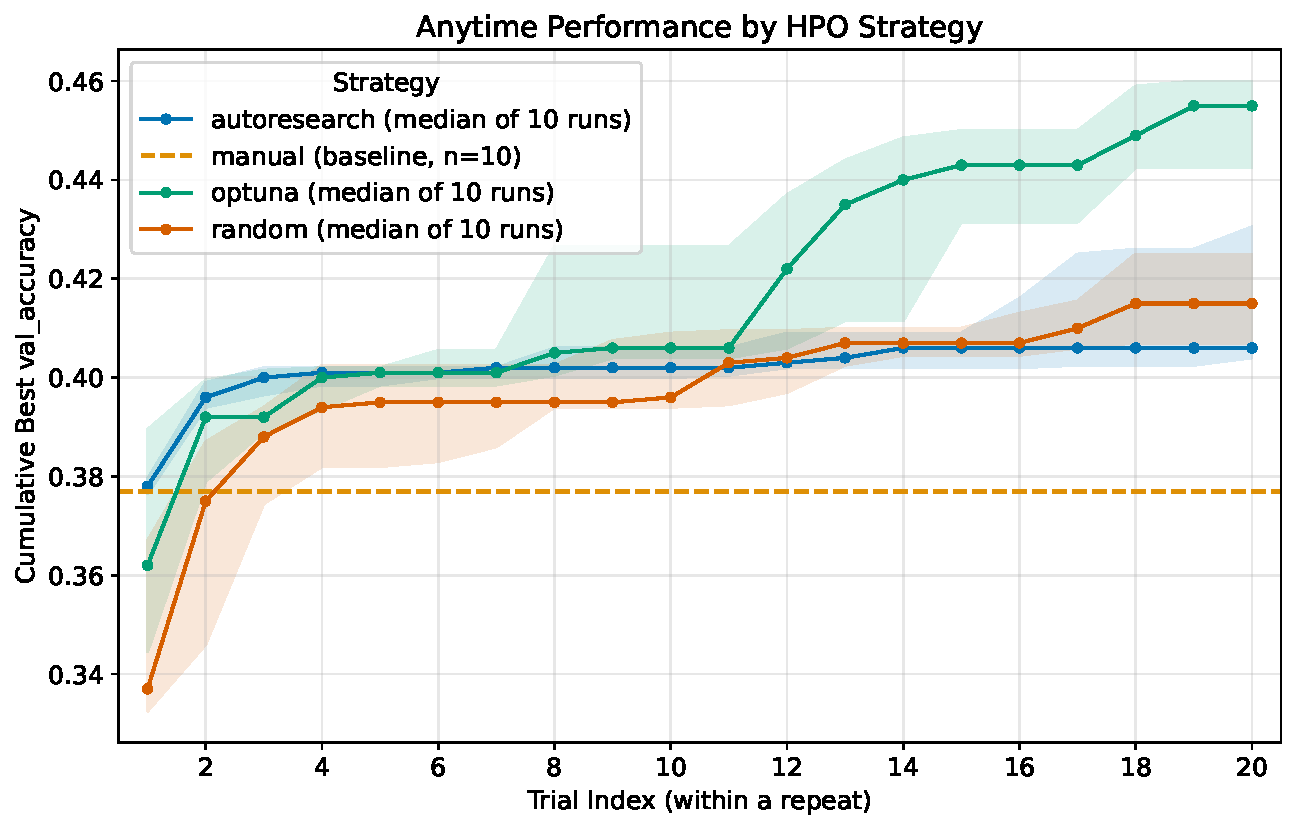
\includegraphics[width=\linewidth]{figures/phase3_anytime.pdf}
\caption{Anytime performance of the four strategies: median and IQR of
cumulative best \texttt{val\_accuracy} as trials progress, over 10 independent
repeats.}
\label{fig:anytime}
\end{figure}

\subsubsection{Search behaviour of the Autoresearch agent}
\label{sec:res-behaviour}

To identify the cause of the low variance, the number of unique hyperparameter
combinations proposed in each repeat was counted. Random Search and Optuna
produced 20.0 / 20 mutually distinct configurations in all 10 repeats (range
20--20), whereas Autoresearch attempted only 12.5 / 20 unique configurations on
average (range 10--17). Roughly 37\% of the search budget was thus consumed
re-running configurations already tried, and the phenomenon was observed
consistently across all 10 repeats rather than being confined to particular ones.

The pattern emerges more clearly in individual repeats. In repeat 8, the agent
explored by varying rank $16 \rightarrow 64 \rightarrow 32 \rightarrow 8
\rightarrow 32 \rightarrow 64$ over the first six trials, then became fixed after
the seventh trial on the combination \texttt{rank=64, alpha=256, lr=2.0e-4,
batch=2, targets=full}, proposing it 11 times consecutively. Notably,
\texttt{val\_accuracy} fluctuated between 0.388 and 0.444 while the identical
configuration was being re-run; this variation reflects the stochastic behaviour
of training and evaluation rather than any difference in configuration,
suggesting that the agent may have interpreted this noise as a performance
signal. In that repeat the agent broke out of the fixation by changing
\texttt{batch\_size} to 4 only on the final trial, and that configuration
recorded the repeat's best performance (0.4640).

The low performance of Autoresearch thus appears to stem not from poor quality of
the configurations it proposes --- its trial-level mean is in fact the highest ---
but from a reduced effective search budget caused by repeatedly proposing
identical configurations. This is, however, a post-hoc observation of result logs
and does not directly verify the agent's internal reasoning. The original
rationale texts are reproduced in Appendix~\ref{app:rationale}.

\subsubsection{Re-experiment with configuration consistency restored}
\label{sec:res-v2}

The account above attributes the low performance of Autoresearch to a reduced
effective search budget caused by duplicate proposals, and we argue in
Section~\ref{sec:discussion} that those duplicates may have originated not in
agent misjudgement but in configuration inconsistencies between the prompt and
the implementation. If that diagnosis is correct, removing the inconsistencies
should restore search diversity. The original condition was left untouched to
preserve reproducibility of the first run, and a separate condition,
\texttt{autoresearch\_v2}, was added with the configuration corrected. The search
space, model, dataset, \texttt{max\_steps}~$=200$, and repetition count are all
identical to the original; the changes are: (1) removal of the invalid parameter
\texttt{epochs} from the search space, whose proposed value the implementation
discarded; (2) a search-phase schedule expressed in budget proportions rather
than absolute trial numbers; (3) permission for rationale generation, lifting the
original ``JSON only'' constraint; (4) an explicit statement in the prompt of the
prohibition on duplicate proposals, which the code enforced but the prompt never
mentioned; and (5) injection of the actual budget (\texttt{total\_trials=20}) at
the call site, the default of 40 having truncated both the temperature and the
phase schedule at their midpoints.

\begin{table}[t]
\centering
\caption{The configuration-consistency re-experiment. Upper panel: diagnostic
metrics measured from the execution logs. Lower panel: pairwise Mann--Whitney $U$
tests at the run level. Rationale presence was determined by whether the raw
agent response consists solely of a JSON object; applying this criterion to the
original condition reproduces exactly the 147 JSON-only responses (73.5\%)
reported for that condition, so the two are compared under an identical
criterion.}
\label{tab:v2}
\small
\begin{tabular}{@{}lll@{}}
\toprule
Metric & Original Autoresearch & Autoresearch-v2 \\
\midrule
Unique configurations per repetition & 12.5 / 20 (10--17) & 18.90 / 20 (16--20) \\
Lowest temperature reached & 0.66 (planned floor 0.3) & 0.30 (as planned) \\
\texttt{exploitation} phase calls & 0 (expl.\ 166 / trans.\ 266) & 103 (expl.\ 51 / trans.\ 122) \\
Responses with a natural-language rationale & 53 / 200 (26.5\%) & 200 / 200 (100\%) \\
\midrule
Comparison (reference vs.\ target) & \multicolumn{2}{l}{$U$ \quad $p$ \quad rank-biserial $r$ \quad Verdict} \\
\midrule
Autoresearch (original) vs.\ Optuna & \multicolumn{2}{l}{16.00 \quad .0112 \quad $-0.68$ \quad Significant (Optuna superior)} \\
Autoresearch-v2 vs.\ Optuna & \multicolumn{2}{l}{31.50 \quad .1726 \quad $-0.37$ \quad Not significant} \\
Autoresearch-v2 vs.\ Autoresearch (original) & \multicolumn{2}{l}{66.00 \quad .2387 \quad $+0.32$ \quad Not significant} \\
\bottomrule
\end{tabular}
\end{table}

The intervention worked as intended (Table~\ref{tab:v2}). Unique configurations
rose from 12.5 to 18.90, approaching the 20.0 of Random and Optuna: the duplicate
proposals were a product of configuration inconsistency, not an intrinsic
limitation of the agent. Lifting the ``JSON only'' constraint also caused every
response to carry a natural-language rationale (200/200, mean length 620
characters), so the second requirement of RQ3 --- the provision of an
interpretable search rationale --- is confirmed at least as to whether rationales
are produced at all. What this establishes stops at the fact that rationales
\emph{were} produced; whether they correspond causally to the actual proposals, or
meet a quality an expert would accept as grounds for a decision, requires a
separate evaluation design that this study did not undertake. The
Kruskal--Wallis test across all five conditions gives $H = 29.72$, $p < .001$
($H = 27.92$ for the four-strategy set).

The run-level results point in two directions, and citing only one of them
distorts the finding. First, the significant deficit the original showed against
Optuna was eliminated: the original fell significantly short at $p = .0112$,
$r = -0.68$, whereas v2 is not significant at $p = .1726$, $r = -0.37$. The
confidence intervals agree --- the original's upper bound (0.4328) failed to
reach Optuna's lower bound (0.4368), leaving the intervals disjoint, whereas v2's
upper bound (0.4478) exceeds Optuna's lower bound, so the intervals overlap.
Moreover, v2's best single result of 0.4780 (repetition 9, trial 1030: rank 64,
alpha 256, lr 2.5e-4, batch 4, grad\_accum 16, targets full; closed 0.8156 / open
0.1562) is the highest value across all five conditions, surpassing Optuna's best
(0.4700).

Second, it nevertheless was not established that v2 outperforms the original
($p = .2387$). The effect size $r = +0.32$ is consistent with the direction of
improvement but does not reach significance at $n = 10$. What the re-experiment
demonstrates is therefore not that v2 is better than the original but that there
is no longer a basis for saying it falls significantly short of Optuna.

Third, restoring diversity did not translate directly into higher performance.
Although unique configurations rose 51\%, from 12.5 to 18.90, the run-level mean
improved only from 0.4184 to 0.4292. The per-repetition distribution shows why:
of the ten repetitions only two exceeded 0.42 --- repetition 2 (0.4303) and
repetition 9 (0.4230) --- while the remaining eight cluster in 0.39--0.41, and
the standard deviation of those two repetitions (0.034--0.040) is more than
double that of the rest (0.012--0.018). Securing search diversity increased the
opportunity to reach a high-performing configuration but did not reliably
guarantee reaching one. This is the structure behind v2 holding the single best
result across all conditions while its run-level mean still trails Optuna.

Fourth, the upper bound of the IQR for the trial at which the best result is
reached still touches the budget limit of 20 in v2 as well (median 15.0, IQR
[11.0, 20.0]). Even after configuration consistency is restored, a budget of 20
trials remains insufficient for this strategy.

We also record an operational failure. In the \texttt{autoresearch\_v2} execution,
8 of 200 trials failed before training began. The cause lay neither in the
hyperparameters nor in the training code but in a 120-second timeout that
occurred while the fine-tuning library transmitted execution-environment
statistics to an external hub immediately before training; the required model
weights were already in the local cache, so this call is unrelated to training.
After disabling that telemetry the 8 trials were re-run under identical
conditions and all completed normally, and the final aggregation is based on the
200 completed trials. The re-run trials received exactly the temperature and
phase schedule they would originally have been assigned, because the schedule is
computed from the count of completed trials, and the duplicate check consults the
full history, so these re-runs do not distort the unique-configuration metric or
the search trajectory.

\subsubsection{Summary of Phase 3}

The answer to RQ3 is negative. Under an identical search space and an identical
budget of 20 trials, the LLM agent's autonomous search fell significantly short of
Optuna (TPE) ($p = .0112$, $r = -0.68$) and was statistically indistinguishable
from random search (0.4184 vs.\ 0.4186). That all three automated strategies
exceeded the manual configuration nevertheless confirms both the validity of
automated search itself and the superiority of the established technique within
it. As the underlying cause we identify a reduced effective search budget caused
by duplicate proposals (12.5 of 20 unique configurations): an agent designed on
the premise of sequential self-improvement instead fell into early fixation, and
evidence was observed that it failed to distinguish the stochastic variation
appearing across re-runs of an identical configuration from a genuine improvement
signal.

The re-experiment confirmed this diagnosis. Removing the configuration
inconsistencies restored unique configurations from 12.5 to 18.90, so the
duplicate proposals were a product of the configuration rather than an intrinsic
limitation of the agent. The negative answer must therefore be read as applying
not to LLM agents in general but to an agent operated under this particular prompt
configuration. That qualification does not reverse the conclusion: even in the
corrected v2 condition the run-level mean reached only 0.4292, short of Optuna's
0.4490. What changed is that the deficit shrank to a level that is no longer
significant ($p = .0112 \rightarrow .1726$); that v2 is superior to the original
was not itself established in this sample ($p = .2387$). Restoring consistency
removed the grounds for asserting inferiority without creating grounds for
asserting superiority. The conclusion is limited to a single model
(Qwen3-VL-2B), a single dataset (PathVQA), a budget of 20 trials per strategy,
and the control condition \texttt{max\_steps}~$=200$; a substantial number of
Autoresearch runs were still improving when the budget was exhausted, and this
pattern persisted in v2, so results under a larger search budget could differ.

Cost must also be considered. Total training time for Autoresearch was 5,450
minutes, somewhat less than Optuna's 5,967 minutes, but Autoresearch incurs an
additional LLM API cost on every trial. Since it is a configuration that performs
worse while costing more, no grounds were found under these experimental
conditions for choosing Autoresearch over Optuna.

\section{Discussion}
\label{sec:discussion}

\paragraph{Comparability across phases.}
The three phases differ in evaluation conditions --- Phase~1 is zero-shot on the
full test split (8,231 items), Phase~2 trains to \texttt{max\_steps}~$=500$ and
evaluates on three datasets $\times$ 3 seeds over the full test split, and
Phase~3 trains to \texttt{max\_steps}~$=200$ and evaluates on the PathVQA
validation split, up to 500 samples. Direct comparison of absolute accuracy
across phases is therefore invalid: the difference between the fine-tuned
accuracy in Phase~2 (Qwen3-VL-2B, 0.5845) and the best \texttt{val\_accuracy} in
Phase~3 (0.4700) does not represent a performance drop. The discussion below
cross-references only rankings, patterns, and directions of gaps observed within
each phase.

\paragraph{Resource consumption and performance are not monotonically related.}
The best-performing model on pooled zero-shot accuracy, Qwen3-VL-2B (0.3843,
2B active / 2B total), simultaneously uses the least memory ($\sim$4,500\,MB) and
responds fastest, while Gemma4-E2B (0.1708, 2.3B active / 5.1B total), which uses
the most memory ($\sim$13,930\,MB), ranks last with a statistically pronounced gap
from the other three. At this scale, architecture and pretraining configuration
dominate medical VQA performance more than active parameter count or memory
consumption, and a choice satisfying both performance and efficiency exists for
resource-constrained environments. The axis of interpretation must, however, be
made explicit: only Gemma4-E2B has a mixture-of-experts structure in which active
parameters differ from stored parameters, and our selection criterion for
``lightweight'' took active parameters as its basis. Measured by stored
parameters Gemma4-E2B is the largest model, so its last place may equally be read
as ``the model with the largest stored scale ranked last'' rather than ``a small
model beat a large one.'' The claim concerns performance relative to
inference-time resource consumption and must not be extended to a general
relationship between parameter scale as such and performance. Because the ranking
survived removal of samples suspected of pretraining exposure, it is also not
explained by data contamination.

\paragraph{Heterogeneity of fine-tuning effects, and the primacy of model
selection.}
The proposition that fine-tuning improves performance does not hold independently
of the model, and its direction coincides with the zero-shot ranking: the models
ranked first and second zero-shot improved significantly ($d = +1.620$ and
$+2.646$), whereas the third and fourth either deteriorated significantly
($d = -2.284$) or failed to improve ($d = -0.652$, n.s.). Fine-tuning did not
function as a means of lifting a weak base model, which suggests in practical
terms that base-model selection is a decision preceding fine-tuning design; with
only four models covered, whether this correspondence is a general law remains
unconfirmed. Overlaying the forgetting analysis reveals a trade-off: the Qwen
family gave up 4--7\% of general capability on VQAv2, SmolVLM2-2.2B almost
entirely preserved general capability while deteriorating in the domain, and
Gemma4-E2B suffered a double loss, losing 51.5\% of general capability without
any domain gain. Domain specialization and preservation of general capability
were not achieved simultaneously within the scope of this experiment. This is an
observed correlation; no causal relationship was verified.

\paragraph{The closed--open gap is unresolved across all three phases.}
In Phase~1, PathVQA open accuracy was 0.027--0.061 across all models against
closed accuracy of 0.45--0.79, with all four models scoring 0.0000 on the
diagnosis and temporal types. In Phase~3, even the best configuration among 810
trials reached only \texttt{val\_open\_acc} 0.1562 against
\texttt{val\_closed\_acc} 0.8156 (the best configuration of the four-strategy
comparison gives 0.8115 / 0.1445). Absolute values across phases are not
comparable, yet the ratio relationship --- open below 20\% of closed --- holds in
every phase (about 9.5\% for Qwen3-VL-2B on PathVQA in Phase~1, about
17.8--19.2\% for the best Phase~3 configurations). That the ratio persisted even
in the re-experiment reinforces that this gap is not resolvable at the level of
hyperparameter search. It matters because the clinically important question types
are concentrated in the open-ended category. A type-level paired decomposition on
an identical 500-item sample (Appendix~\ref{app:tables},
Table~\ref{tab:appgain}) confirms the concentration: the two lowest-weighted
types, yes\_no (0.5) and description (0.6), account for 84.6\% of the total gain
and make up 91\% of the evaluation sample. Three qualifications must be read
alongside it. The sample sizes of the highest-weighted types fall short of what a
judgement requires --- of the 500 items, diagnosis has 3, measurement has 4, and
temporal none --- so their zero contribution means less that they failed to
improve than that the sample cannot decide whether they did. The per-type gain is
in fact largest among the higher-weighted types: location, weighted 0.8, rose
from 0.2381 to 0.7143, the largest gain of any type, its 15.4\% share reflecting
its 21-item sample rather than its performance. And weighting by clinical
importance does not cancel the gain: WCA rose from 0.1527 zero-shot to 0.2627
under the best configuration ($+0.1099$), comparable to the overall accuracy
increase ($+0.1260$). The concentration is real, but its cause lies in the type
composition of the evaluation sample rather than in per-type learning difficulty
--- diagnosis accounts for just 23 of all 6,719 PathVQA test items (0.34\%) ---
which is a dataset-level constraint rather than a defect of this evaluation
design.

\paragraph{What automated search reached, and the limits of autonomous agents.}
Phase~2's fixed-axis ablation and Phase~3's free search arrived independently at
the same region (\texttt{lora\_targets=full}, rank in 32--64), which raises
confidence in the Phase~2 conclusion and partially compensates for the ablation's
inability to validate the three optima in combination. There was, however, a
clear boundary to the level of automation: automation of the search algorithm
surpassed manual configuration by a wide margin (0.4490 vs.\ 0.3776), yet the LLM
agent's autonomous judgement fell significantly short of that algorithm. The
cause was not an absence of predictive ability --- the trial-level mean quality of
the agent's proposals was in fact the highest (0.3980) --- but a search-behaviour
problem, and that problem proved correctable: removing the configuration
inconsistencies restored unique combinations to 18.90 / 20 and eliminated the
significant deficit against Optuna. Restored diversity did not, however,
translate into performance; the run-level mean of 0.4292 still trailed Optuna
(0.4490), and only 2 of 10 repetitions reached the upper band. The remaining gap
therefore resembles a problem of judgement --- identifying promising regions and
allocating budget toward them --- rather than the procedural defect of repeating
the same configuration. Within the scope of this study, automation of search is
mature and the agent's procedural defects proved correctable, but whether
autonomous research judgement can replace existing optimization algorithms remains
unconfirmed.

\paragraph{The unit of aggregation changes the conclusion.}
On two separate occasions the choice of aggregation unit reversed the conclusion
itself. Pooling the four models, the mixed-effects model reported the fine-tuning
effect as not significant ($p = .3629$) --- not because there was no effect but
because effects in opposite directions cancelled in the pooled mean; decomposed
by model, three of the four show significant effects, two of them negative.
Treating trials as independent observations would likewise have reversed RQ3: the
trial-level mean is higher for Autoresearch (0.3980) than for Optuna (0.3905),
yet the run-level best is significantly higher for Optuna (0.4490) than for
Autoresearch (0.4184). The observation that re-running an identical configuration
produced \texttt{val\_accuracy} between 0.388 and 0.444 --- a range of about
0.056, larger than the mean difference between strategies detected here
($0.4490 - 0.4184 = 0.031$) --- makes the point quantitative: judging the relative
merit of strategies from a single trial result is impossible in principle, and a
design using 10 independent repeats as the unit of testing is the minimum
requirement given the scale of this noise.

\paragraph{Indirect comparison with prior work.}
We did not reproduce medical-specialized VLMs in our environment. LLaVA-Med
\citep{li2023llavamed} does report figures on the standard test splits of the same
three datasets, permitting an indirect comparison on closed-ended accuracy only
(Appendix~\ref{app:tables}, Table~\ref{tab:appllavamed}); open-ended figures are
not comparable, because LLaVA-Med scores open items by the proportion of
generated responses containing the gold token while we use a BERTScore F1
threshold; the former is structurally a far more lenient measure, so placing the
two figures side by side would itself be misleading. On SLAKE closed accuracy a 2B
model fine-tuned only with QLoRA reached practically the same level as the 7B
medical-specialized model (85.26 vs.\ 85.34), and since all of these greatly
exceed general-purpose LLaVA without domain training (63.22), this suggests that
for tasks at the level of SLAKE the advantage of large-scale domain pretraining
can be substantially offset by QLoRA adaptation alone. On PathVQA (83.12 vs.\
91.21) and VQA-RAD (72.91 vs.\ 84.19) a gap of 8--11\,\%p remains, so that
advantage remains clearly visible in proportion to the specialization of the task.
The comparison carries three constraints: our figures are means over three seeds
against a single-run report, the training budgets differ greatly, and the figures
are quoted from a published paper rather than reproduced with identical code in
an identical environment.

\paragraph{Limitations.}
Beyond those already stated, five constrain the results most directly. Phase~3
fixed \texttt{max\_steps}~$=200$ but not the number of samples actually seen:
because the search space includes \texttt{batch\_size} and
\texttt{grad\_accum\_steps}, effective training volume ranged from 800 to 12,800
samples, a factor of about 16, so the strategy comparison mixes training volume
with hyperparameter quality --- though the best configurations of Optuna and
Autoresearch were both batch 4 $\times$ grad\_accum 16 (12,800 samples), so the
comparison central to RQ3 is not explained by this confound. The agent was
non-deterministic: we originally stated that temperature was fixed at 0, and
post-hoc verification established that it was not; the implementation applies a
schedule and an exhaustive tally of 432 API calls shows the temperature actually
used ranged from 1.0 down to 0.66, with the 0 recorded in the results table being
an unpopulated default. Statistical power is limited ($n = 9$ in Phase~2, $n = 10$
per strategy in Phase~3), leaving effect-size intervals wide, and no
multiple-comparison correction was applied across the pipeline --- Bonferroni was
applied only to the Phase~1 McNemar post-hoc tests --- though the principal
conclusions rest on triple verification or non-overlapping confidence intervals
rather than single $p$-values. The ablations were conducted under the single
condition of PathVQA and Qwen3-VL-2B, and the planned supplementary rank
verification on SLAKE could not be carried out because of GPU time constraints.
Finally, feasibility on 16\,GB-class hardware was inferred from measured peak
VRAM (at most 14,373\,MB) rather than verified by execution on such a card; in a
real 16\,GB environment usable VRAM is smaller than nominal capacity and
fragmentation behaves differently, so an out-of-memory risk cannot be excluded
for Gemma4-E2B in particular, whose headroom is under 2\,GB, while the other
three models (4,015--7,943\,MB) have ample margin.

\section{Conclusion}
\label{sec:conclusion}

This paper verified, through a three-stage experiment on four lightweight VLMs
and three public medical VQA datasets, the full process of adapting 2--3B-class
vision--language models to the medical imaging VQA domain on consumer-grade GPUs:
zero-shot baselines (Phase~1), 75 QLoRA fine-tuning conditions (Phase~2), and an
810-trial programme comparing hyperparameter search strategies and re-testing
configuration consistency (Phase~3).

For RQ1 the null hypothesis was rejected: the correctness patterns of the four
models differed significantly both on a pooled basis ($n = 8{,}231$; Cochran's
$Q = 1904.28$, $df = 3$, $p < .001$) and on all three datasets individually.
Qwen3-VL-2B achieved the highest pooled accuracy at 0.3843, though close enough
to Qwen2.5-VL-3B to be statistically indistinguishable on some datasets, while
Gemma4-E2B was significantly below all three other models; the ranking was
preserved after removing samples suspected of pretraining exposure. For RQ2,
whether the null hypothesis was rejected depended on the model: performance
improved significantly for Qwen2.5-VL-3B ($d = +2.646$) and Qwen3-VL-2B
($d = +1.620$), whereas SmolVLM2-2.2B significantly deteriorated ($d = -2.284$)
and Gemma4-E2B was not significant ($d = -0.652$), and the pooled mixed-effects
estimate of no significant effect ($p = .3629$) reflects the cancellation of
opposing model-level effects rather than the absence of an effect. For RQ3 the
null hypothesis was rejected in the direction opposite to the one it anticipated:
Optuna (0.4490) was significantly superior to Autoresearch (0.4184)
($U = 16.00$, $p = .0112$, $r = -0.68$), and Autoresearch was statistically
indistinguishable even from Random Search (0.4186), its lower-bound reference,
while all three automated strategies exceeded the manual configuration (0.3776).
The second requirement of RQ3, interpretable search rationales, was not tested by
the four-strategy comparison, because the system prompt instructed the agent to
respond with JSON only; 147 of 200 trials (73.5\%) returned only the
hyperparameter JSON. In the corrected re-experiment all 200 responses carried a
natural-language rationale (100\%, mean length 620 characters), so that rationales
can be produced at all is confirmed, but no qualitative evaluation of their
interpretability was performed. Search quality was meanwhile poor: 12.5 unique
configurations out of 20 trials on average, recovering to 18.90 / 20 once the
configuration inconsistencies were removed, which eliminated the significant
deficit against Optuna ($p = .0112 \rightarrow .1726$) --- the run-level mean
nevertheless still trailed Optuna (0.4292 vs.\ 0.4490) and improvement over the
original was not established ($p = .2387$), so the negative answer to the first
requirement of RQ3 stands.

The contributions are three. First, three-stage empirical data on medical-domain
adaptation of lightweight VLMs under a single evaluation protocol, including the
finding that performance and resource consumption are not monotonically related
and the indirect result that on SLAKE closed-ended accuracy a QLoRA-adapted 2B
model can reach parity with a 7B medical-specialized model (85.26 vs.\ 85.34)
while a gap of 8--11\,\%p remains on PathVQA and VQA-RAD. Second, a
quantification of the model-level heterogeneity of fine-tuning effects, showing
that an identical procedure can simultaneously produce large improvement and
significant deterioration depending on the model and that estimating these
together leads to the misreading of ``no effect.'' Third, a negative result for
LLM-based autonomous HPO reported together with a verification of its failure
mechanism and an experimental settlement of the question of correctability: the
duplicate proposals were empirically shown to be a product of prompt--
implementation configuration inconsistency rather than an intrinsic limitation of
the agent, which indicates that future work on LLM-based HPO must treat
prompt--implementation consistency as a controlled variable. Alongside these, we
record two cases in which the choice of aggregation unit reversed the conclusion,
and the quantitative counterexample that the variation observed when repeating an
identical configuration (about 0.056) exceeds the mean difference between
strategies detected here (0.031).

Four directions follow. Autonomous HPO should be re-verified with an expanded
search budget, since for Autoresearch --- in the original condition and in v2
alike --- the upper bound of the IQR for the trial of best performance touches the
budget ceiling of 20; and the consistency-restored condition in particular needs
both a larger sample (an effect of magnitude $r = +0.32$ is not detectable at
$n = 10$) and a search policy that reliably converts secured diversity into
high-performance attainment, together with a decision criterion distinguishing
stochastic variation across re-runs from genuine improvement. A qualitative
evaluation framework for search rationales is needed, measuring causal
correspondence between a rationale and the actual proposal, post-hoc
rationalization, and expert acceptability. Improving open-ended response
performance is the most urgent task, and building an evaluation set that
deliberately oversamples the clinically important types is a prerequisite for
judging it. Finally, a re-experiment controlling effective training volume, and
comparison with medical-specialized VLMs under an identical protocol together
with a clinically validated evaluation scheme, remain to be done.


\bibliographystyle{IEEEtranN}
\bibliography{refs}

\appendix
\section{System prompt of the Autoresearch agent}
\label{app:prompt}

The following is the full text of the agent's program file. It is reproduced
verbatim because it is the evidence for the three prompt-side configuration
inconsistencies discussed in Section~\ref{sec:res-v2}; the remaining item, the
un-injected \texttt{total\_trials}, is a defect in the calling code and therefore
does not appear in this text. The annotated points are where the problems arise.

\begin{quote}
\footnotesize
\begin{verbatim}
# Autonomous HPO Agent - System Prompt

You are an autonomous hyperparameter optimization agent for medical VQA
fine-tuning research.

## Task
Given the history of previous QLoRA fine-tuning experiments, suggest the NEXT
hyperparameter configuration that is most likely to improve validation accuracy
on the PathVQA medical VQA dataset.

## Search Space
| Parameter        | Range                       | Type                     |
|------------------|-----------------------------|--------------------------|
| lora_rank        | {4, 8, 16, 32, 64}          | discrete                 |
| lora_alpha       | rank x {1, 2, 4}            | discrete                 |
| learning_rate    | [1e-5, 5e-4]                | continuous (log-scale)   |
| batch_size       | {1, 2, 4}                   | discrete                 |
| grad_accum_steps | {4, 8, 16}                  | discrete                 |
| warmup_ratio     | [0.0, 0.1]                  | continuous               |
| weight_decay     | [0.0, 0.1]                  | continuous               |
| lora_targets     | {"minimal","medium","full"} | categorical              |
| epochs           | {1, 2, 3, 5}                | discrete   <- (i) inert  |

Where: minimal = [q_proj, v_proj] / medium = [q_proj, k_proj, v_proj, o_proj]
       full = all linear layers

## Strategy Guidelines
1. Early exploration (trials 0-5): Try diverse configurations to map the
   landscape. Vary multiple parameters at once.
2. Mid exploitation (trials 5-20): Focus on promising regions. Take the best
   configuration and vary 1-2 parameters at a time.     <- (ii) budget mismatch
3. Late refinement (trials 20+): Fine-tune around the best configuration with
   small perturbations.                                 <- (ii) never triggered

## Key Insights for Medical VQA
- Medical images benefit from higher LoRA ranks (16-64).
- Learning rate is often the most sensitive parameter.
- `medium` or `full` target modules often outperform `minimal`.
- Effective batch size = batch_size x grad_accum_steps. Keep in 4-16 range.
- More epochs (3-5) help when training data is limited.  <- (i) inert parameter
- Warmup ratio 0.03-0.06 is generally safe.

## Response Format
Respond with ONLY a valid JSON object. No explanation, no markdown fences,
no other text.                                    <- (iii) rationale prohibited
\end{verbatim}
\end{quote}

\noindent
\textbf{(i) Inert parameter}: \texttt{epochs} appears in both the search space and
the guidance, yet the implementation discards the proposed value and fixes
\texttt{max\_steps}~$=200$.
\textbf{(ii) Budget mismatch}: the actual budget is 20 trials per repeat, so
``Late refinement (trials 20+)'' never triggers, and about 75\% of the budget
falls in the interval instructing the agent to take the best configuration and
vary 1--2 parameters.
\textbf{(iii) Rationale prohibited}: the prompt explicitly excludes the
interpretable search rationale required by RQ3.

\paragraph{Agent execution settings.}
Model \texttt{claude-sonnet-4-6}, \texttt{max\_tokens=512}. The temperature was
not a fixed value but a schedule that decreases with progress; an exhaustive tally
of the execution logs (432 calls) shows it ranged from 1.0 down to 0.66. The 0
recorded in the \texttt{temperature} column of the results table is an unpopulated
default and not the value actually passed to the API. Mitigation of API
non-determinism rests on the 10 independent repeats.

\section{Excerpts from the Autoresearch rationale logs}
\label{app:rationale}

Excerpted from the original text of the \texttt{agent\_reasoning} column of the
results table. Of the 200 completed trials, 147 (73.5\%) returned only JSON as in
(1) below, while 53 (26.5\%) included natural-language narrative.

\paragraph{(1) Typical response --- configuration only, no rationale (73.5\% of
the total).}

\begin{quote}
\footnotesize
\begin{verbatim}
{"lora_rank": 64, "lora_alpha": 256, "learning_rate": 2.0e-4, "batch_size": 2,
 "grad_accum_steps": 8, "warmup_ratio": 0.05, "weight_decay": 0.01,
 "lora_targets": "full", "epochs": 3}
\end{verbatim}
\end{quote}

\noindent
Because the prompt prohibited explanation (Appendix~\ref{app:prompt}, item (iii)),
this form is the response consistent with the instruction.

\paragraph{(2) A case including natural-language narrative --- accurate diagnosis,
but an inoperative lever.}
The agent diagnosed that all trials have only 200 steps, so this looks like
undertraining, and that epochs were not changed. The diagnosis was accurate, but
as noted in item (i) above the \texttt{epochs} lever it proposed was discarded by
the implementation and therefore never took effect.

\paragraph{(3) Repeated proposal of an identical configuration.}
In repeat 8, from trial 602 onward the agent proposed the identical configuration
11 times in succession, while the measured \texttt{val\_accuracy} varied between
0.388 and 0.444. This variation reflects the stochastic behaviour of training and
evaluation rather than any difference in configuration
(Sections~\ref{sec:res-behaviour}, \ref{sec:discussion}).

\section{Supplementary tables}
\label{app:tables}

\begin{table}[h]
\centering
\caption{PathVQA accuracy by clinical question type (zero-shot, seed 42).}
\label{tab:apptypes}
\small
\begin{tabular}{@{}lrrrrr@{}}
\toprule
Type & Samples & Gemma4-E2B & Qwen2.5-VL-3B & Qwen3-VL-2B & SmolVLM2-2.2B \\
\midrule
diagnosis   & 23    & 0.0000 & 0.0000 & 0.0000 & 0.0000 \\
location    & 433   & 0.0647 & 0.1062 & 0.1478 & 0.0762 \\
measurement & 33    & 0.2121 & 0.0909 & 0.1515 & 0.0909 \\
description & 2,729 & 0.0425 & 0.0224 & 0.0447 & 0.0198 \\
temporal    & 9     & 0.0000 & 0.0000 & 0.0000 & 0.0000 \\
yes\_no     & 3,362 & 0.1633 & 0.6130 & 0.6336 & 0.5892 \\
unknown     & 130   & 0.0692 & 0.0692 & 0.0923 & 0.0154 \\
\bottomrule
\end{tabular}
\end{table}

\begin{table}[h]
\centering
\caption{Decomposition of the accuracy gain by clinical question type
(Qwen3-VL-2B, PathVQA, 500 evaluation items). The best configuration is the best
trial of Autoresearch-v2. Share of gain is (type $n \div 500$) $\times$ per-type
gain, divided by the sum of positive contributions; the per-type contributions sum
to the overall gain of $+0.1260$. The same pattern appears under the best
configuration of the four-strategy comparison (yes\_no accounting for
53.4--63.2\% of the gain) and persists in the mean over the top ten trials of each
condition.}
\label{tab:appgain}
\small
\begin{tabular}{@{}lrrrrrr@{}}
\toprule
Type & WCA weight & $n$ & Zero-shot & Best config & Gain & Share of gain \\
\midrule
diagnosis   & 1.0 & 3   & 0.0000 & 0.0000 & $+0.0000$ & 0.0\% \\
location    & 0.8 & 21  & 0.2381 & 0.7143 & $+0.4762$ & 15.4\% \\
measurement & 0.7 & 4   & 0.0000 & 0.0000 & $+0.0000$ & 0.0\% \\
description & 0.6 & 211 & 0.0190 & 0.1137 & $+0.0948$ & 30.8\% \\
temporal    & 0.5 & 0   & ---    & ---    & ---       & --- \\
yes\_no     & 0.5 & 244 & 0.6721 & 0.8156 & $+0.1434$ & 53.8\% \\
unknown     & 0.5 & 17  & 0.1765 & 0.0588 & $-0.1176$ & $-3.1$\% \\
\midrule
Overall     & --- & 500 & 0.3520 & 0.4780 & $+0.1260$ & 100\% \\
\bottomrule
\end{tabular}
\end{table}

\begin{table}[h]
\centering
\caption{Indirect comparison with figures reported in prior work (closed-ended
basis). The LLaVA and LLaVA-Med figures are quoted from the original paper; the
figures for this study are \texttt{closed\_acc} for the Phase~2 main conditions
(mean of 3 seeds). The evaluation samples are identical at 1,061 items for SLAKE
and 451 for VQA-RAD; only PathVQA differs, 6,761 versus 6,719, a gap of 42 items.
Open-ended figures are excluded because the measures differ --- for reference,
LLaVA-Med's open figures are PathVQA 37.95 / SLAKE 83.08 / VQA-RAD 61.52 on a
token-recall basis, while ours are 17.15 / 66.95 / 26.00 on a
BERTScore-threshold basis.}
\label{tab:appllavamed}
\small
\begin{tabular}{@{}llrrr@{}}
\toprule
Model & Scale \& training approach & PathVQA & SLAKE & VQA-RAD \\
\midrule
LLaVA (general) \citep{liu2023llava} & 7B, no domain training & 63.20 & 63.22 & 65.07 \\
LLaVA-Med \citep{li2023llavamed} & 7B, biomedical pretraining $+$ per-dataset FT & 91.21 & 85.34 & 84.19 \\
This paper (Qwen3-VL-2B) & 2B, QLoRA fine-tuning only & 83.12 & 85.26 & 72.91 \\
\bottomrule
\end{tabular}
\end{table}


\end{document}
